\documentclass[a4paper,polish,12pt]{article}
    \usepackage[utf8]{inputenc}
    \usepackage[T1]{fontenc}
    \usepackage{lmodern}
	\usepackage{amsmath}
	\usepackage{xcolor}
    \usepackage{babel}
    \usepackage{csquotes}
    \DeclareQuoteAlias{croatian}{polish}
    \usepackage[%
    style=verbose-ibid, % numeric, alphabetic, authoryear, ect.
    sorting=nty,
    isbn=false,
    abbreviate = false,
    backend=biber,]{biblatex}

    \renewcommand*{\newunitpunct}{\addcomma\space}
    \renewbibmacro*{in:}{}

    \usepackage{xpatch}

    \xpatchbibdriver{book}{%
    \newunit
    \iffieldundef{maintitle}
    {\printfield{volume}%
    \printfield{part}}
    {}%
    }
    {%
    }{}{}

    \xpatchbibdriver{book}{%
    \usebibmacro{publisher+location+date}%
    }
    {%
    \usebibmacro{publisher+location+date}%
    \newunit
    \printfield{volume}%
    \printfield{part}
    \usebibmacro{finentry}
    }{}{}

    \DeclareFieldFormat{journaltitle}{\mkbibquote{#1}}
    \DeclareFieldFormat[article,periodical]{number}{nr.  #1}% number of a journal

    \DeclareFieldFormat
    [article,inbook,incollection,inproceedings,patent,thesis,unpublished]
    {title}{\mkbibemph{#1}}
    %
    \renewbibmacro*{journal+issuetitle}{%
    \usebibmacro{journal}%
    \setunit*{\addspace}%
    \iffieldundef{series}
    {}
    {\newunit
    \printfield{series}%
    \setunit{\addspace}}%
    \usebibmacro{issue+date}%
    \setunit{\addspace}%
    \usebibmacro{issue}%
    \setunit{\addspace}%
    \usebibmacro{volume+number+eid}%
    \newunit}

    \renewbibmacro*{issue+date}{%
    \iffieldundef{issue}
    {\usebibmacro{date}}
    {\printfield{issue}%
    \setunit*{\addspace}%
    \usebibmacro{date}}%
    \newunit}

    \renewbibmacro*{publisher+location+date}{%
    \printlist{publisher}%
    \iflistundef{publisher}
    {\setunit*{\addcomma\space}}
    {\setunit*{\addcomma\space}}%
    \printlist{location}%
    \setunit*{\addspace}%
    \usebibmacro{date}%
    \newunit}
\usepackage{graphicx}
\usepackage{color}

\usepackage{listings}
 \renewcommand{\lstlistingname}{kod} %zmiana podpisu na polski

\definecolor{dkgreen}{rgb}{0,0.6,0}
\definecolor{gray}{rgb}{0.5,0.5,0.5}
\definecolor{mauve}{rgb}{0.58,0,0.82}


\lstset{frame=tb,
 language=Python,
 aboveskip=3mm,
 belowskip=3mm,
 showstringspaces=false,
 columns=flexible,
 basicstyle={\small\ttfamily},
 numbers=none,
 numberstyle=\tiny\color{gray},
 keywordstyle=\color{blue},
 commentstyle=\color{dkgreen},
 stringstyle=\color{mauve},
 breaklines=true,
 breakatwhitespace=true,
 tabsize=3
}

\usepackage{hyperref}
\newtheorem{theorem}{Twierdzenie}
\addbibresource{bik.bib}
\newtheorem{tw}{Twierdzenie}
\title{Projekt Cyfrowe przetwarzanie sygnałów}
\date{}
\author{Szymon Kozakiewicz}

\title{Repeta sieci}

\begin{document}
\maketitle
\section{Ad hoc and Sensor Networks: Motivation and Applications}

\subsection{What are disadvantages of infrastructure-based wireless networks and what are possible solutions ?}

\subsubsection{Wady seici opartych na infrastrukturze}
\begin{itemize}
\item możliwy lokalny brak infrastruktury(gdzieś na pustyni)
\item zbyt drogie lub trudne stworzenie infrastruktury (ponownie pustynia)
\item brak czasu na stworzenie infrastruktury(np podczas wojny)
\end{itemize}
\subsubsection{Możliwe rozwiązania(alternatywy)}
\begin{itemize}
\item użycie sieci ad hoc(rozumiem że te niżej to jej przykłady)

\item mobilona infrastruktura(centrum łączności jest jakiś pojazd np czołg)
\item komunikacja między samochodami(na zasadzie peer to peer)
\item Systemy search-and-rescue przydatne podczas lawin
\item Personal area networking(używane przez zegarki, urządzenia medyczne, smart opaski itp)

\end{itemize}

\subsection{What are problems and challenges for networks (like ad hoc network) without a central infrastructure ?}


\begin{itemize}
\item Brak centralnej jednostki zarządzającej siecią(np zasobami, routingiem )
\item ograniczony zasięg nadajników w urządzeniach użytkowych
\item mobilność nadajników(częsta zmiana sąsiedztwa, dróg routingu itp). im większa grupa puczestników sieci tym trudniej
\item niektóre nadajniki są zasilane baterią co moze doprowadzać do ich nagłego wyłączenia, skracać czas działania sieci.
\end{itemize}
\subsection{Explain the notions of „sources“, „sinks“ and „actuators“ in wireless sensor networks (WSN) ?}

\begin{description}
\item[sources] źródła dancyh, zwykle mowa o sensorach
\item[sinks]\textit{Zlew} Zbiera dane od sensorów
\item[Actuators]Kontroluje urządzenia(nie wiem czy chodzi o sensory czy o jakies urządzenia nie należące do sieci) w oparciu o spływające z sieci dane. Często również jest to sink
\end{description}

\subsection{What is a concept of WSN with a central control}
\textcolor{red}{Do tego była jedna ilustracja}:\ref{zdj:centralControl}.
\begin{figure}

\caption{}
\label{zdj:centralControl}
\centering
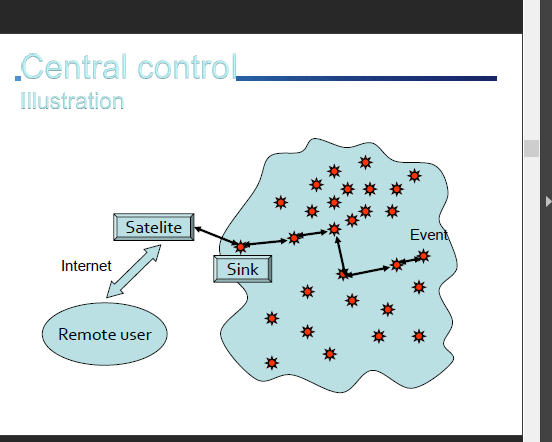
\includegraphics[width=\textwidth]{zdjecia/centralControl}
\end{figure}

\subsection{What is a concept of autonomous WSN}
\begin{itemize}
\item Sink jest mobilny
\item mozliwa komunikacja na znacznych dystansach(\textcolor{red}{za pomocą udogodnień?})
\item udstepnia interfejs dla zewnetrznego użytkownika
\item \textcolor{red}{Napisane jest duża iloośc energi(tyle pali czy co?)}

\item może byc aplikowane na polach bitewnych, w sytuacjach kryzysowaych 
\end{itemize}
Ilustracja: \ref{zdj:answer}.
\begin{figure}

\caption{}
\label{zdj:answer}
\centering
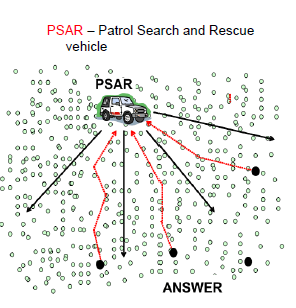
\includegraphics[width=\textwidth]{zdjecia/answer}
\end{figure}
\subsection{What is wearable computing}
Chodzi o ubrania napakowane sensorami i wysyłające różne informacje(temperatura ciała np). przykład UbiComp: Microsoft’s Doll
\subsection{Describe applications of WSN in ecology monitoring (e.g. in animal monitoring (Great Duck Island).)}
\begin{itemize}
\item Mozna monitorowac zachowania lęgowe ptaków()
\item wykrywać pożary lasów
\item wykrywać ataki chemiczne i biologiczne
\item Eksperyment Redwood Tree, rzociągnieto 10km kabli żeby zbadać klimat na różnych wysokościach drzewa
\end{itemize}
\subsubsection{Great Duck Island)}
\begin{itemize}
\item umieszcano czujniki w podziemnych gniazdach
\item były również czujniki nad gniazdami umiesznone na 10 cm nóżkach
\item dane z senosorów były transmitowane do stacji badawczej a z niej poprzez satelite do zainteresowanych naukowców
\end{itemize}
\subsection{Describe applications of WSN in precision agriculture and intelligent buildings/bridges.}
\begin{itemize}
\item sensory można rozkłądać na polu by monitorować mikroklimat(temperature,wilgotność, nawożeniem, poziom użycia pestycydów)
\item dzięki temu precyzyjnie można aplikować pestycydy lub nawadnaić i generuje to duze oszczednosci.
\end{itemize}


\subsection{What are structuring types of WSN applications}
%Nie wiem czy dobrze zrozumiałem pytanie ale takie slajdy były. 
%\begin{itemize}
%\item śledzenie dostarczyciela sensorów
%\begin{itemize}
%\item dostarczyciel to np samolot
%\item wyrzuca on sensory w odpowiedniej kolejności
%\item dzięki GPs samolotu wiedzą one mniej wiecej gdzie się znajduja(te sensory)
%\end{itemize}
%\item smart parkingi(prowadzenie klienta do wolnego miejsca parkingowego, sprawdzanie którym samochodom minął czasi mozna im dać mandat)
%\item monitorowanie konstrukcji(np mostów) czyb się nie rozpadają
%\item wirtulane ogrodzenia dla krów(pastuchy). Jak krowa wyjdzie pozaa wyznaczony obszar to jest rażona prądem 
%\item inteligentne budynki
%\item monitorowanie dzikiej przyrody
%\item inteligentne budynki
%\end{itemize}


\begin{description}
\item[Wykrywanie zdarzeń] 
\item[okresowe pomiary]
\item[Aproksymacja funkcji] np pomiar temperatuyry w czasie/przestrzeni
\item[wykrywanie krawędzi jakiegoś kształtu]
\item[śledzenie]  np samolotu
\end{description}
\subsection{What are deployment/maitenance options for WSN}
\subsubsection{Opcje dostarczania sensorów}
\begin{itemize}
\item losowe rozstawienie, zwykle używny jest uniform distribution
\item regular deployment. Jest planownay i stały, zwykle rozkład jest geometryczny
\item sensory mobilne
\begin{itemize}
\item mogą zmienaić pozycje same lub z pomocą jakieś siły np wiatru
\item potrafi aktywnie wyszukiwać interesujące obszary
\end{itemize}

\end{itemize}
\subsubsection{Opcje utrzymania}
\begin{itemize}
\item wymiana baterii
\item\textcolor{red}{praca bez nadzoru}?(unattended operation?)
\item ładowanie słoneczne
\end{itemize}
\subsection{What are characteristic requirements for WSN ?}

\begin{itemize}
\item Musi brać problemy z byciem w zasięgu geograqficznym(issues like geographic scoping are natural requirements, absent)
\item \textcolor{red}{Powinno pozwalać na przesyłanie odpowiedzi(a nie tylko liczb)}
\item przesyłanie bitów nie jest tak proste jak w innych sieciach
\item tradycyjne metryki QoS nie mogą byc aplikowane
\item usłga WSN musi być \textit{dobra} czyli oferwać dobre odpowiedz w dobrym czasie
\item duża odpornośc na błedy(węzły moga byc nagle niszczone, wyłaczać sie z braku energi)
\item sieć powinna działac tak by maksymalizowac swój czas zycia
\item skalowalność(musi byc wsparcie dla wielu węzłów)
\item Wspomagać różne poziomy gestości węzłów na jednostke powieszchni
\item Udostepnaić możliwość przeprogramwoania węzłow
\item WSN musi adaptować sie do zmian, sama siebie monitorować, móc dołączać nowe zasoby(np dodatkowo zrzucone sensory)
\end{itemize}
\subsection{What are required mechanism to meet requirements ?}
\begin{itemize}
\item Multi-hop wireless communication
\item Wszystkie operacje wykonywane w sieci powinny uwzględniać oszczędzanie energii.
\item Auto konfiguracja sieci(raczej nie manualna)
\item jesli to mozliwe w sieci powinnien obywać się preprocesing dancyh
\item Węzły w sieci powinny współpracowac w celu osiągniecia wspólnego celu
\item Data centric networking(patrz dalej)
\item lokalność działań, jak najwiecej działań powinno być robione lokalnie
\item architektóra sieci powinna byc kompromisem miedzy dokładnością a efektywnością energetyczną.
\end{itemize}
\subsection{Explain the notion „data centric networking“}
W takiej sieci w głównej mierze skupiamy się na dancyh a nie jak konkretnie beda rozstawione węzły w przestrzeni.
\subsection{What are the main differences between Ad Hoc and WSN networks ?}
\textcolor{red}{MANET=Ad Hoc?}
\begin{itemize}
\item MANET jest potężniejszy(i droższy), wystepuje w nich wiekszy przepływ danych, jest wiecej zasobów.
\item to jak wygląda WSNs mnocno zależy od tego jaka jest aplikacvja która ma obsługiwać, MANET jest bardziej uniwersalny
\item \textcolor{red}{Rdzeń wsn nieobecny w MANET}
\item wsn mogą być wieksze
\item WSN są bardziej oszczędne energetycznie
\item Rózna mobilność(in WSN sinki mogą byc mobilne a wezły musza byc stacjonarne)
\item WSN są data centryczne a MANET id-centryczne(id-centric)


\end{itemize}
\section{Physical Layer – Wireless Basics}

\subsection{What are the main functions of Physical Layer in OSI Model ?}

Funkcje warstwy fizycznej
\begin{itemize}
\item wykonuje usługi dal warstwy łacza danych(data link)
\item \textcolor{red}{Zajmuje się fizycznymi aspektami intefejsu i mediów}
\item odpowiada za reprezentacje bitów, czestotliowść transmisji, synchronizacje bitów
\item konfiguracja połacazenia
\item fizyczna topologia 
\end{itemize}

\subsection{What are differences between OSI Model and TCP/IP Model ?}
\begin{itemize}
\item OSI jest starszy
\item nowoczesne systemu raczej korzystają z TCP
\item Osi ma 7 warstw a TCP  4. Wastwa aplikacji TCP/ip reprezentuje 3 inne warstwy OSI

\end{itemize}
\subsection{What are differences between analog and digital signals ? Give examples of analog signals.}
sygnał analogowy przyjmuje wartości rzeczywiste a sygnał cyfrowy dyskretne(0,1).
\subsubsection{Przykłady}
temperatura, ciśnienie,sygnał radiowy
\subsection{Explain in words the main parameters of sinusoid wave.}
\subsubsection{Aplituda}
maksymalne wychylenie od poziomu 0
\subsubsection{częstotliwość}
Częstotliwośc to liczba pełnych przebiegów fali w ciągu 1 sekundy
\subsubsection{Faza}
jeżeli mają tą samą faze to powinny mieć te samą wartość w punkcie (0,0)(tak to profesor tłumaczył)
\subsubsection{Okres}
czas, jendego pełnego przebiegu fali
\subsubsection{Długośc fali}
droga przeyta przez fale w czasie 1 okresu. wzór $\lambda=vT$  gdzie T to okres a v to prędkośc fali
\subsection{What is a formal relation (equation) between wavelength and frequency ?}
$\lambda=\frac{v}{f}$
\subsection{Calculate a period of a wave of the length 1 mm.}
$\frac{\lambda}{v}=\frac{0.001}{300 000 000}$
Nie wiem czy to dobrze, zakładam predkość fali na prędkość swiatła, pamietam ze uzywaliśmy jej na wykładzie.
\subsection{Explain what kind of activity....}
\begin{description}
\item[zasieg interferencji]słyszymy tylko szumy
\item[Zasięg detekcji]adresat bedzie miedział że coś jest wysyłane ale nie bedzie w stanie wiedział co
\item[zasięg transmisji]
jest pełna funkcjonalność
\end{description}
\subsection{What is attenuation between 10 and 100 meters distance, attenuation by such objects as textile or concrete wall ?}
nie jestem penwy czy o to chodzi
\begin{description}
\item[textile]3dB
\item[concentrate walls] 13-20 dB

\end{description}


\subsection{What are mechanisms of wave propagation and how they influence on it ? How power of a signal received from transmitter depends on a distance d ?}
\begin{description}
\item[Refleksja] powodowana przez obiekty które są wieli w porównaniu z długością fali
\item[Dyfrakcja]Powodowana przez obiekt o nieregularnych kształtach który jest miedzy odbiorcą a nadawcą
\item[rozpraszanie] Powodowane jest przez obiekty które są mniejsze niż długość fali.
\end{description}
Siła sygnału maleje z kwadratem odległości


\subsection{What is Doppler shift ?}
Z wykładu: Random frequency modulation


Z wkipedii:zjawisko fizyczne występujące dla fal, polegające na powstawaniu różnicy częstotliwości fali wysyłanej przez jej źródło oraz częstotliwości fali rejestrowanej przez obserwatora(zwykle spowodowane jest to ruchem źrodła lub odbiorcy sygnału).



\subsection{How path loss depends on a frequency of a signal ?}
Im wyższa częstotliwość tym szybciej sygnał wygaszany jest przez odległość
\subsection{What is a delay spread ?}

Echo sygnału. najpierw do uzytkownika dolatuje pierwotny sygnmał a potem (lub jednoczesnie) sygnał który gdzieś tam się odbijał (patrz obrazek \ref{zdj:delay}).
\begin{figure}

\caption{}
\label{zdj:delay}
\centering
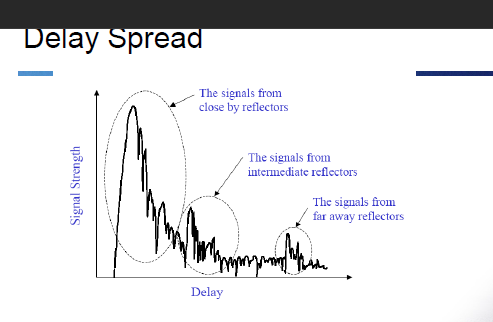
\includegraphics[width=\textwidth]{zdjecia/delay}
\end{figure}
\subsection{What is intersymbol interference ?}
Jeśli sygnał odbity i sygnał źródłowy się nakładaja(Niektóre bity moga też wcale nie dochodzić lub dochodzić  z opóźnieniem) może dochodzić do błędów (patrz \ref{zdj:delay}). 
\begin{figure}

\caption{}
\label{zdj:}
\centering
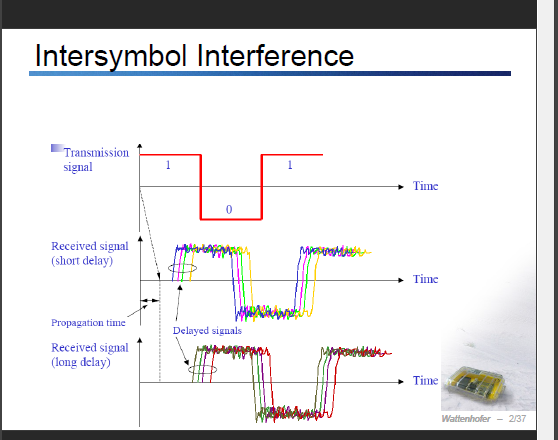
\includegraphics[width=\textwidth]{zdjecia/intersymbol}
\end{figure}
\section{Multiple Division Techniques}
\subsection{what is a purpose of multiplexing}

multiplexing to transmitowanie wielu sygnałów za pomocą tego samego medium(za pomocą jedengo kabla)
\subsection{what are dimensions of multiplex channels and what is their influence on multiplexing ?}
\begin{itemize}
\item przestrzeń(space(s))
\item czas time(t)
\item częstotliwość(f)
\item code(c)
\end{itemize}
Można używac ponownie niektore częstotliwości dopiero w pewnej odległości od innej stacji bazowej ktora też używa tej samej częstotliwości

\subsection{how the problem of multiplexing is solved in cellular networks}
jeśli spadek siły sygnału przez dystans jest conajmniej 9db to jest ok

\subsection{what is a concept of FDMA ?}
Frequency division Multiple access. Dzielimy spektrum częstotliowści na częsci(channele). Każdą część dostaje jakis uzytkownik i może jej uzywać(patrz rysunek \ref{zdj:FDMA}). Technologia stara, nieleastyczna. Plus jest taki ze pracuje z sygnałami analogowymi.
\begin{figure}

\caption{}
\label{zdj:FDMA}
\centering
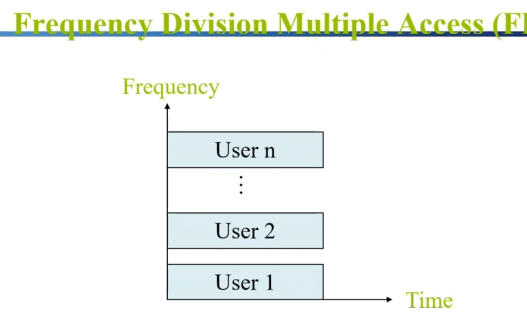
\includegraphics[width=\textwidth]{zdjecia/FDMA}
\end{figure}

\subsection{what is a concept of TDMA}
Time division Multiple access.Użytkownik dostaje dla siebie całe spektrum częstotliowści ale na krótki okres czasu (milisekundy). Obrazek \ref{zdj:TDMA}. Tak naprawdę zamiast jednego usera jest grupa userów która korzysta z przypisanych sobie czestotliwości tak jak to było FDMA(ale lepiej mowic w razie czego że topn jedna osoba ma całe spektrum ma jedna osoba bo tak jest na jego obrazkach). używane przez systemy drugiej generacji(GSM). 
\begin{figure}

\caption{}
\label{zdj:TDMA}
\centering
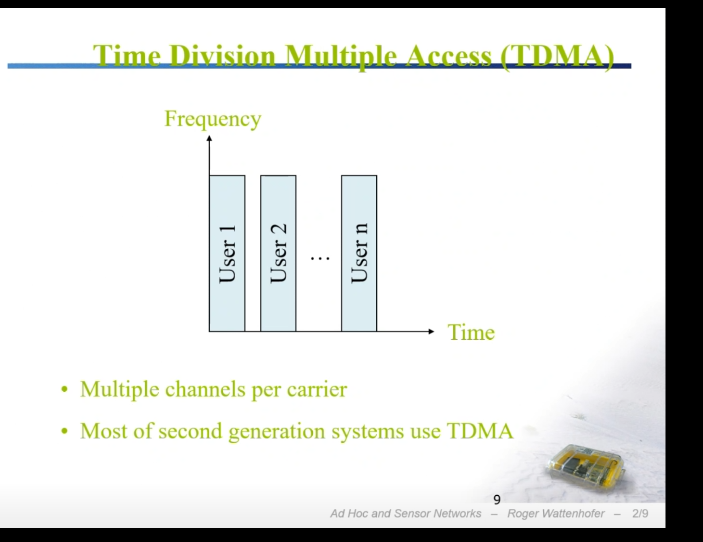
\includegraphics[width=\textwidth]{zdjecia/TDMA}
\end{figure}
\subsection{what is a concept of CDMA}
Względem poprzednich typów dodano dodatkowy wymiar:code. Wszyscy uzytkwnicy moga uzywac czestotliwosci w tym samym czasie poniewaz używają innego kody(?).


\subsection{what is analogy between coctail party and multiplexing ?}

\begin{itemize}
\item przestrzeń multiplaxingu to komunikacja między róznymi pokojami
\item częstątliwość to używanie różnych tonów(sopran,alt, tenor itp)
\item czas multiplex. W jednym czasie gada jedna osoba mówi. pozwalamy żeby inny rozmówca skończył 
\item code miltiplex, jest jak używanie róznych języków. Łatwiej wyłowić własny język z gwaru rożnych innych języków

\end{itemize}
\textcolor{red}{Dalej jest do kolosa numer 2}
\subsection{how many channels are requested for communication between 2 clients}



\subsection{what is a concept of frequency hopping ?}



\subsection{what is a modulation ?}



\subsection{what is idea of amplitude modulation ?}



\subsection{what is idea of frequency modulation}

\subsection{what is a concept of digital modulation called Amplitude Shift Keying}



\subsection{what is a concept of digital modulation called Frequency Shift Keying}



\subsection{what is a concept of digital modulation called Phase Shift Keying ?}



\subsection{what is the idea of UWB modulation ?}



\subsection{what is the idea of OFDM modulation ?}

\end{document}